\section{Benefits}
\begin{table}[htbp]
  \centering
  \caption{Overview of capacitive proximity sensing benefits}
    \begin{tabular}{p{4cm}p{6cm}}
    \toprule
    \textbf{Name} & \textbf{Examples} \\
    \midrule
    \textbf{Versatility} & Flexible electrode design, scalability, different sensing methods \\
    \textbf{Unobtrusiveness} & Invisible application, non-disturbing frequency range \\
    \textbf{Processing Complexity} & Small number of sensors, variable dynamic range \\
    \bottomrule
    \end{tabular}%
  \label{tab:cap_benefits}%
\end{table}%

After discussing the various limitations of capacitive proximity sensing, the following section will give an overview of the benefits.  Similar to the previous section we have three groups, namely versatility, unobtrusiveness and processing complexity. Some examples within these groups are shown in Table 6.
\subsection{Versatility}
A main benefit of capacitive proximity sensing is the versatility in which they can be applied. The flexibility of electrode materials, size and geometry allows specifically creating highly individual applications. Example electrodes include transparent metal oxide layers, woven conductive thread, copper wires, PCB boards or simple aluminum foil. 
The sensors systems are also highly scalable. By choosing appropriate voltages and frequencies it is possible to add a high number of sensors to a single object. Using smart measurement windows and different multiplexing methods, sensors can be placed close together and electrodes may act as both sender and receiver.
The different sensing methods presented - loading mode, shunt mode and transmit mode enable a variety of different sensing patterns. The human body can be used as both sender and receiver and smart electrode layouts allow using a smaller number of processing units. 
In conclusion, it is possible to add capacitive sensing to most everyday objects to enable different forms of interaction, create natural interfaces and smart objects. Our prototypes are using different electrode materials, flexible or solid electrodes, conductive thread, wires, shielded or non-shielded layouts. 
\subsection{Unobtrusiveness}
 \begin{figure}[h]
\centering
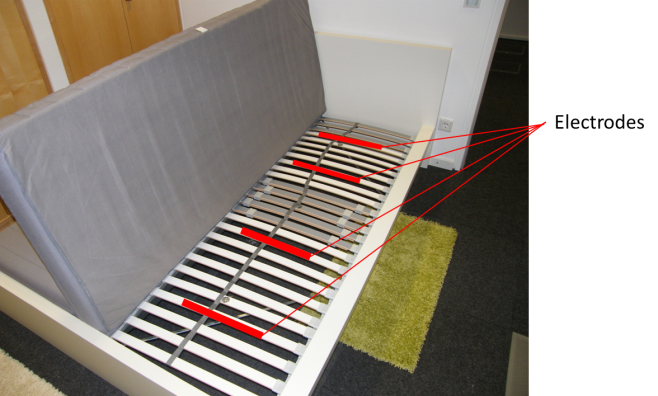
\includegraphics[width=0.6\textwidth]{images/disc_unob_bed.png}
\caption{Electrodes and sensors hidden below mattress of Smart Bed}
\label{fig:disc_unob_elec}
\end{figure}
Electric fields are not usually perceived by persons, unless they are of exceptional strength. Furthermore they propagate through many materials that we are typically using in our environment, including most plastics, wood or tiles. This allows us to invisibly apply capacitive proximity sensors without a strong effect on the measurement. Application below several centimeters of covering is possible, if the electrodes are designed properly for sensing in this distance.
The frequency range in which the sensors are operating is usually not in an interval that disturbs other electronic systems. Thus it is feasible to use capacitive sensing even in environments, where non-disturbance is a main requirement.  Additionally the used frequencies are not considered to be biologically active, and good results can be achieved using small currents. 
It is possible to equip most conductive objects directly with capacitive proximity sensors and hide them below non-conductive objects with minimal spatial requirements. Our Smart Bed and Active Armrest prototypes are using sensor sets that are completely invisible from the outside and communicate wirelessly to a PC only using a power supply. Figure \ref{fig:disc_unob_elec} shows the electrodes and sensors hidden below the mattress of the Smart Bed.
\subsection{Processing Complexity}
An appropriate analogy of capacitive proximity sensors is a single photodiode. As opposed to a light intensity we are measuring capacitance. While the information we can gain from such a measurement is limited, the processing required to analyze the signal is also low. Performing signal analysis on an array of 16 capacitive sensors is comparable to processing the image of a 4x4 pixel camera. Therefor it is easy to create highly integrated systems with very low-power devices for performing any subsequent data analysis. While it is possible and in many cases beneficial to use complex data processing algorithms for object detection it is in most cases still possible to replace them with simpler methods for a comparable result.
In many applications it is even viable to opt for a quantized capacitance measurement. In the case of a touch sensor a single binary measure is sufficient. However, it is also possible to select various different levels and reduce the dynamic range to an easily computable value that is 4 or 8 Bit long. Depending on the chosen algorithm this dynamic range reduction can occur either in pre-processing or high level processing.
With the exception of the Capacitive Chair our prototypes are using simple data processing methods that can be easily applied on embedded systems. A preferred method for object localization is the weighted average algorithm. Regarding model-based data processing, even very simple cylindrical models, such as the one used for the Smart Bed, are capable to reliably predict numerous postures that are relevant in real world applications. In general, the low requirements for data preprocessing, allows dedicating more resources to high level data processing algorithms if the specific application is resource con-strained. 
The OpenCapSense toolkit that is the base for most of our prototypes has a fairly powerful micro-controller that is able to implement all of the processing steps - thus enabling highly integrated, low-power capacitive proximity sensing prototypes that can be used in smart environment applications.